\section{Theorie}
\label{sec:Theorie}
  Der Lock-In-Verstärker ist ein Verstärker, der in der Messung stark verrauschter
  Signale eingesetzt wird, indem das Signal von Störfrequenzen bereinigt wird.
  Er hat einen phasenempfindlichen Gleichrichter integriert.
  \begin{figure}
    \centering
    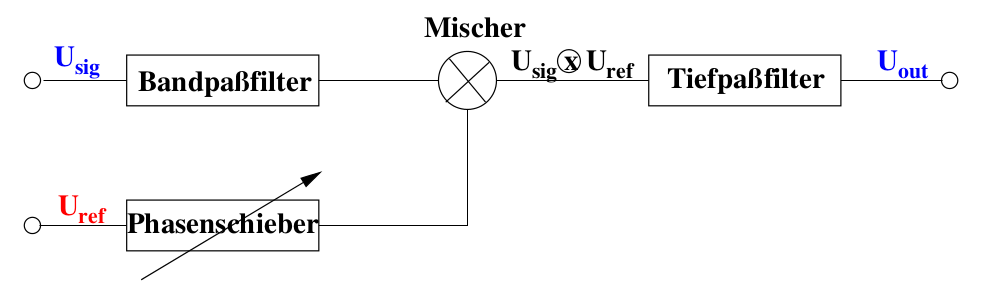
\includegraphics[width=0.7\textwidth]{aufbau.png}
    \label{fig:aufbau}
  \end{figure}
  Der schematische Aufbau eines Lock-In-Verstärkers ist in Abbildung \ref{fig:aufbau}
  zu sehen.
  Das verrauschte Nutzsignal $U_\symup{sig}$ wir mit einer Referenzfrequenz $\omega_0$
  moduliert. Dann werden mit einem Bandpassfilter Rauschanteile mit höherer oder
  niedrigerer Frequenz als $\omega_0$ rausgefiltert.
  Es wird nun ein Referenzsignal $U_\symup{ref}$ mit Frequenz $\omega_0$ erzeugt,
  welches im Mischer mit dem Eingangssignal $U_\symup{sig}$ multipliziert wird.
  Damit die beiden Signale synchron sind (also eine Phasenverschiebung
  $\Delta\Phi=0$ haben), kann die Phasenlage $\Phi$ des Referenzsignals mit einem
  Phasenschieber verändert werden.
  Nach dem Mischer wird das resultierende Signal $U_\symup{sig} \times U_\symup{ref}$
  mit einem Tiefpassfilter über mehrere Perioden integriert. Dabei mitteln sich
  die Frequenzbeiträge, die nicht synchron zur Modulationsfrequenz sind, raus.
  Am Ausgang erhält man damit eine Gleichspannung, welche proportional zur
  Eingangspannung $U_\symup{sig}$ ist. Es gilt $U_\symup{out}\propto U_0 cos\Phi$.
\cite{sample}
